
\subsection{Run and Event Selection}

This thesis analyzes collisions of polarized protons recorded by the STAR
experiment during the years 2005 and 2006. A total of \(11.5~pb^{-1}\) of
longitudinally polarized data were recorded in $\sim$ 1800 STAR runs. The STAR
run serves as the basic unit of quality assurance; if a run fails any part of
the QA procedure the entire run is excluded from further analysis. The QA
metrics considered in this analysis are listed in Table~\ref{tab:qa-metrics}. A
run is rejected if its value for any metric falls more than 3$\sigma$ away from
the mean of that metric's distribution. In addition, any runs shorter than 2
minutes are automatically discarded. Table~\ref{tab:dataset-luminosities}
records the fraction of runs and integrated luminosity that survive this
procedure.

The global track DCA metric is of particular interest.
Figure~\ref{fig:dca-before} shows the initial time-series distribution of this
metric for the 2006 data. The spike around run index 625 corresponds to a purge
of the P10 gas in the TPC. The drift velocity in the TPC was varying rapidly
during this period, and the standard procedure for recording drift velocity
entries in the Calibrations DB for each laser run proved insufficient to track
the variation. A second analysis of the laser data was able to extract
additional drift velocity measurements and parameterize the exponential drop in
drift velocity during the five day period following the purge, as shown in
Figure~\ref{fig:dv-fit}. Finally, Figure~\ref{fig:dca-after} shows the track DCA
distributions after the recalibration of the drift velocity.

\begin{table}
  \centering
  \begin{tabular}{|c|}
    \hline
    Quality Assurance Metrics \\
    \hline
    $z$ position of event vertex \\
    BBC coincidence timebin \\
    global track DCA to the primary vertex \\
    number of jets per event \\
    number of towers per jet \\
    number of tracks per jet \\
    jet $p_T$ \\
    jet tower $p_T$ \\
    jet track $p_T$ \\
    \hline
  \end{tabular}
  \caption{Distributions analyzed in the QA procedure.}
  \label{tab:qa-metrics}
\end{table}

\begin{figure}
  \subfloat[][Before DV Recalibration]{
    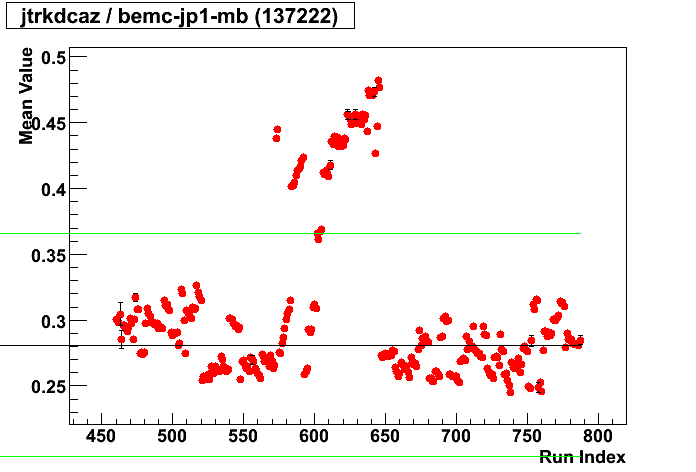
\includegraphics[width=0.5\textwidth]{figures/dca-before}
    \label{fig:dca-before}
  }
  \subfloat[][After DV Recalibration]{
    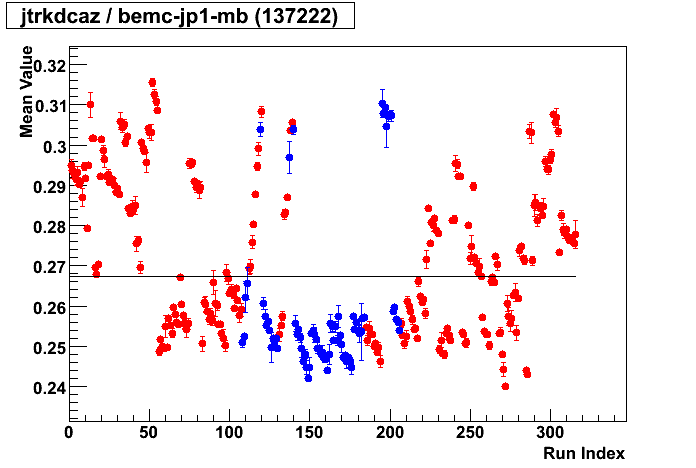
\includegraphics[width=0.5\textwidth]{figures/dca-after}
    \label{fig:dca-after}
  }
  \caption{Global track DCA distributions as a function of time before and after the drift velocity recalibration.  The horizontal green lines in (a) indicate the 3$\sigma$ cut before recalibration.}
\end{figure}

\begin{figure}
  \centering
  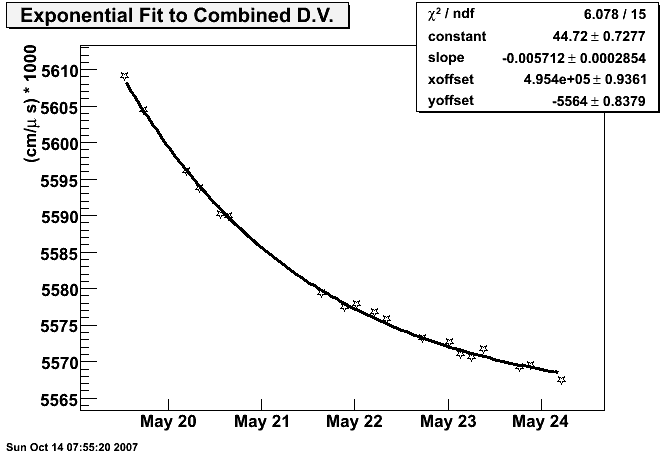
\includegraphics[width=0.7\textwidth]{figures/dv-fit}
  \caption{Parameterization of additional drift velocity measurements allowing for fine-granularity tracking of the TPC drift velocity in the days following the P10 gas purge.}
  \label{fig:dv-fit}
\end{figure}

Events in the runs surviving QA are selected for analysis if a) the event fired
a jet patch trigger, b) the spin states of both beams have been successfully
identified for the bunch crossing, and c) the event vertex position established
from the BBCs is within a selection window.

\begin{table}
  \centering
  \begin{tabular}{|c|cc|}
    \hline
    Time Period & Runs & $\mathcal{L}^{-1} (pb^{-1})$ \\
    \hline
    2005/04/17 - 2005/06/24  & 739/1387 & 2.22/3.77 \\ % ppProduction running
    % 2006/03/12 - 2006/04/06  & 0/447    & 0.00/2.45 \\ % ppProduction (Long1)
    2006/05/12 - 2006/06/05  & 297/464  & 5.59/7.74 \\ % ppProductionLong (Long2)
    \hline
  \end{tabular}
  \caption{Datasets analyzed in this work.  Each cell lists the ratio of accepted data to recorded data for the period in question.}
  \label{tab:dataset-luminosities}
\end{table}

\subsection{Pion Identification}

Charged pions are identified from the subset of primary tracks in each event
having at least 25 fit points, a distance of closest approach (DCA) to the
primary vertex of no more than 1 centimeter, a pseudorapidity magnitude less
than 1.0, and a transverse momentum greater than 2.0 GeV/c. The first three cuts
select high quality tracks. The transverse momentum cut is not necessary from an
experimental perspective, but an \(A_{LL}\) analysis of low momentum pions
offers limited physics insights and the analysis can proceed more efficiently if
these very common particles are not included. The determination of the PID
acceptance window is discussed in Section~\ref{sec:pid} and the window
boundaries are listed in Table~\ref{tbl:pid-selection-windows}.
Figure~\ref{fig:pid-accept-window} highlights the characteristic relativistic
rise of the MIP distribution for the accepted charged pion tracks.

\begin{table}
  \centering
  \begin{tabular}{|c|c|}
    \hline
    Criterion & Efficiency \\
    \hline
    $|\eta| < 1.0$ & 0.94 \\
    at least 25 fit points & 0.95 \\
    $|DCA|$ of associated global track $<$ 1.0 cm & 0.96 \\
    \hline
  \end{tabular}
  \caption{Quality cuts imposed on the high-$p_T$ primary tracks before PID selection.}
\end{table}

\begin{figure}
  \centering
  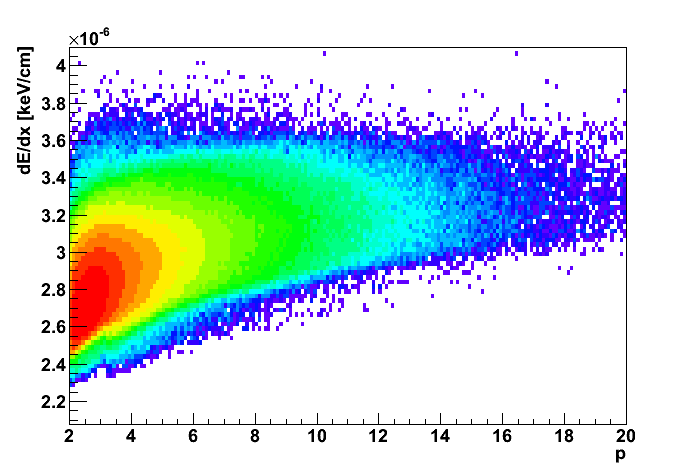
\includegraphics[width=0.7\textwidth]{figures/dEdx_p}
  \caption{Energy loss per unit path length versus momentum for tracks produced by identified charged pions.}
  \label{fig:pid-accept-window}
\end{figure}

\subsection{Jet-Pion Correlations}

In the 2006 data analysis events are accepted only if they contain a
reconstructed jet with an uncorrected \(p_T\) between 10 and 30 GeV/c, a
pseudorapidity between -0.7 and 0.9, and an electromagnetic energy fraction not
greater than 0.92. Furthermore, the difference in azimuth between the jet axis
and the center of a jet patch above the trigger threshold must be no more than
\(36^\circ\). Multiple jets in an event can satisfy these ``trigger jet'' cuts.

Charged pions satisfying the track quality and PID cuts described in the
preceding section are compared against the list of trigger jets. If a charged
pion is separated from a trigger jet by at least 2.0 radians in azimuth it is
considered to be an ``away-side'' pion and is accepted for analysis.
Figure~\ref{fig:dphi} plots the azimuthal distribution of charged pions relative
to trigger jets in the 2006 analysis. The data show good agreement with Monte
Carlo simulations.

\begin{figure}
  \centering
  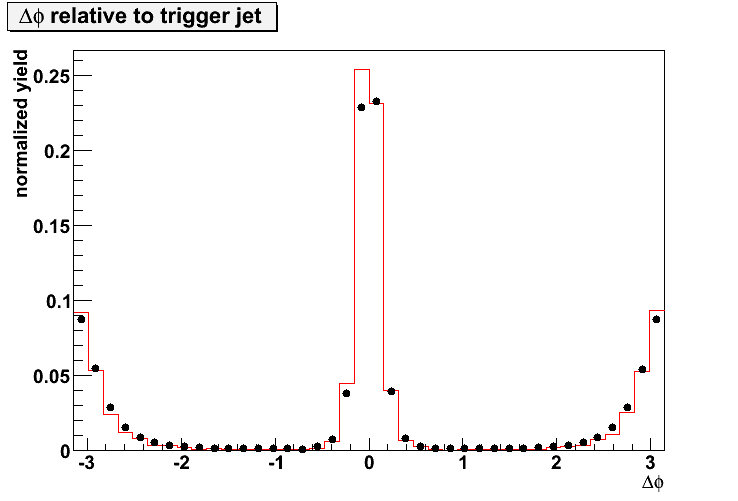
\includegraphics[width=0.7\textwidth]{figures/dphi}
  \caption{Azimuthal distribution of charged pions relative to the trigger jet axis in the 2006 dataset.  The black circles represent data, the red lines fully reconstructed Monte Carlo. Pions with $|\Delta \phi| > 2.0$ are accepted for analysis.}
  \label{fig:dphi}
\end{figure}

The data are binned as a function of \(z\), defined as the ratio of the
away-side pion \(p_T\) and the trigger jet \(p_T\). Figure~\ref{fig:meanpt}
shows that the jet \(\langle p_T \rangle\) is approximately constant as a
function of \(z\), and thus that the charged pion \(\langle p_T \rangle\)
increases linearly with \(z\). Again, the data are modeled well by STAR's
Pythia+GEANT simulations.

\begin{figure}
  \centering
  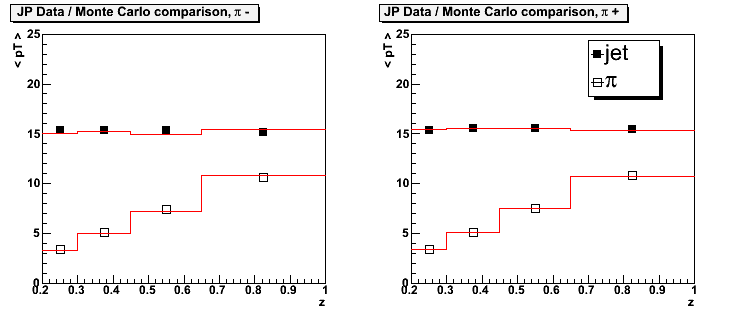
\includegraphics[width=1.0\textwidth]{figures/meanpt}
  \caption{Comparison of the $\langle p_T \rangle$ values for jets and charged pions in each $z$ bin.  The data show good agreement with fully reconstructed Pythia+GEANT events that pass a simulation of the BJP2 trigger.}
  \label{fig:meanpt}
\end{figure}
